\begin{figure}[h]
    \centering
    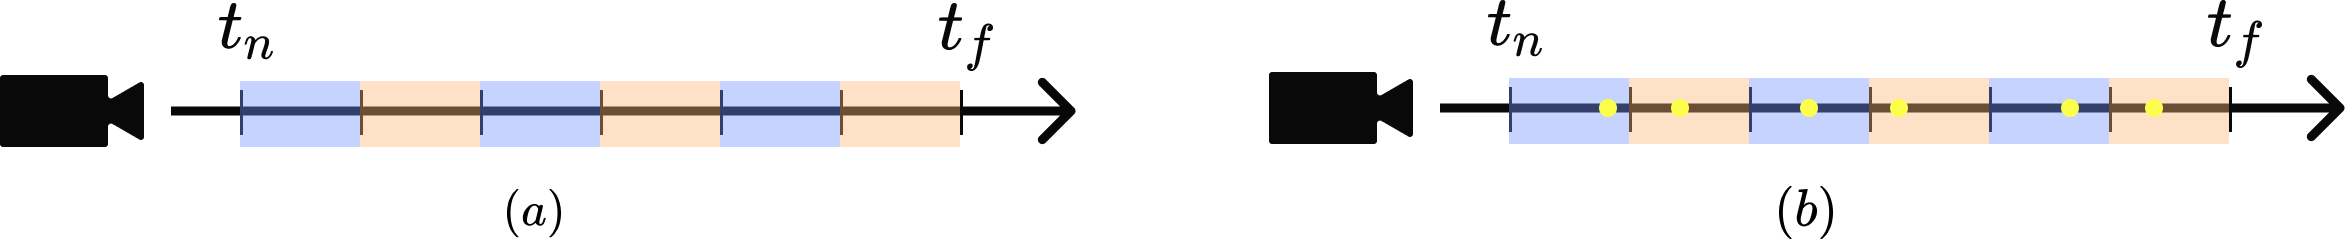
\includegraphics[width=1.0\textwidth]{figures/StratifiedSampling.png}
    \caption{a) The ray is uniformly binned from the near bound $t_n$ to the far bound $t_f$, defining the strata. b) random points are sampled from the bins.}
    \label{fig:stratified-sampling}
\end{figure}